\documentclass[margin=5mm, tikz]{standalone}
\usepackage[utf8x]{inputenc}
\usepackage{tikz}
\begin{document}
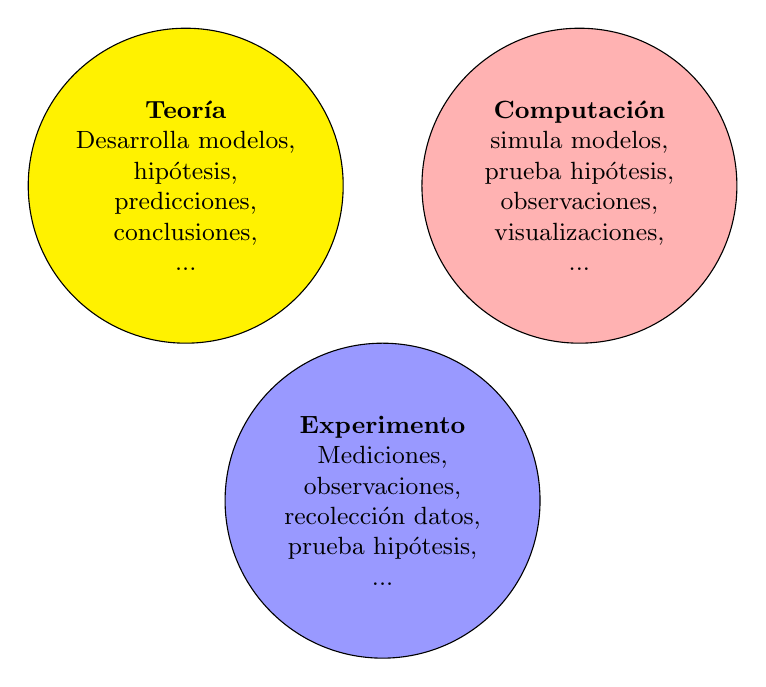
\begin{tikzpicture}[font = \small]
    \draw [fill=yellow, thin] (0, 3.5) circle (2);
    \draw [align=center] (0, 3.5) node {\textbf{Teoría} \\ Desarrolla modelos, \\ hipótesis, \\ predicciones, \\ conclusiones, \\ ...};

    \draw [fill=red!30, thin] (5, 3.5) circle (2);
    \draw [align=center] (5, 3.5) node {\textbf{Computación} \\ simula modelos, \\ prueba hipótesis, \\ observaciones, \\ visualizaciones, \\ ...};

    \draw [fill=blue!40, thin] (2.5, -0.5) circle (2);
    \draw [align=center] (2.5, -0.5) node {\textbf{Experimento} \\ Mediciones, \\ observaciones, \\ recolección datos, \\ prueba hipótesis, \\ ...};
\end{tikzpicture}
\end{document}